% Created 2024-06-07 Fri 16:42
% Intended LaTeX compiler: pdflatex
\documentclass[11pt]{article}
\usepackage[utf8]{inputenc}
\usepackage[T1]{fontenc}
\usepackage{graphicx}
\usepackage{subcaption} % For subfigures
\usepackage{longtable}
\usepackage{wrapfig}
\usepackage{rotating}
\usepackage[normalem]{ulem}
\usepackage{amsmath}
\usepackage{amssymb}
\usepackage{capt-of}
\usepackage{hyperref}
\usepackage{minted}
\usepackage{parskip} % Removing indenting in new paragraphs
\hyphenpenalty=100000 % preventing splitting of words
\author{Nada Dandachi}
\date{\today}
\title{README}
\hypersetup{
 pdfauthor={Nada Dandachi},
 pdftitle={README},
 pdfkeywords={},
 pdfsubject={},
 pdfcreator={Emacs 28.2 (Org mode 9.5.5)}, 
 pdflang={English}}
\begin{document}

\maketitle
\tableofcontents
\clearpage

%_____________________________________________________________%
%_____________________________________________________________%

\section{Installation}
\label{sec:org8bb410e}

%_____________________________________________________________%

\subsection{Prerequisites}
\label{sec:org81d40dc}

Install \textbf{VirtualBox}, an open-source virtual machine emulator available online:
\url{https://www.virtualbox.org/wiki/Downloads}

%_____________________________________________________________%

\subsection{Create the virtual machines (VMs)}
\label{sec:org1b35f14}

In the terminal, launch the \texttt{manual\_install.sh} file in the root of the \texttt{package\_wehe} directory. 
\begin{minted}[]{sh}
    sh wehe_demonstrator/script/manual_install.sh
\end{minted}

If you encounter the following error:
\begin{minted}[]{sh}
    vboxdrv kernel module is not loaded
\end{minted}

Execute the following commands in the terminal:
\begin{minted}[]{sh}
    uname -r
    yum install kernel-devel-<uname -r>
\end{minted}


%_____________________________________________________________%

\subsection{Install Ubuntu on the VMs}
\label{sec:org7b66673}

Start VirtualBox, then launch each of the virtual machines by double clicking on it. Follow the instructions to install Ubuntu (Figure \ref{fig:UbuntuInstall}), this operation takes some time (\textasciitilde{}30 minutes per machine). 

\begin{figure}[H]
  \centering
  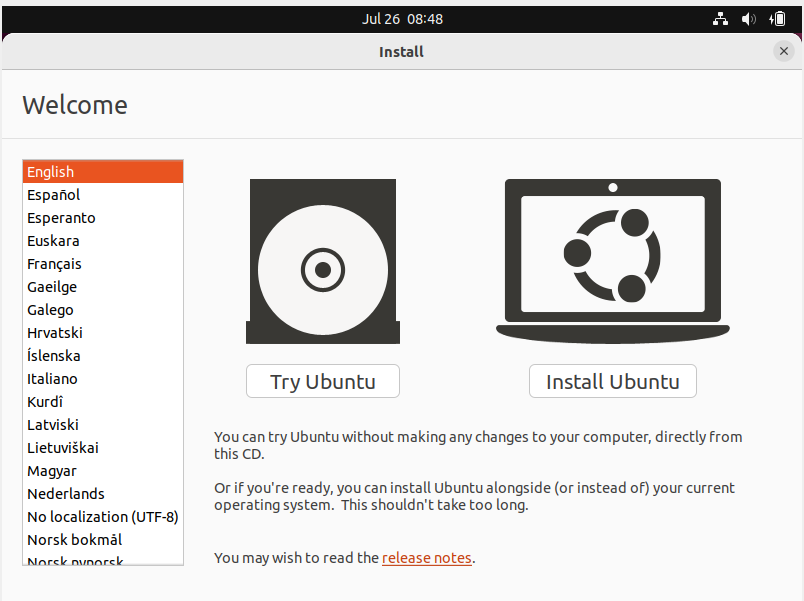
\includegraphics[width=.8\linewidth]{./Images/install_page.png}
  \caption{Install page}
  \label{fig:UbuntuInstall}
\end{figure} 


Name the virtual machines server, client and middlebox. 
\begin{itemize}
    \item The username for the server VM will be "server" and the password will be "Server" (Figure \ref{fig:LoginPage}).
    \item The username for the client VM will be "client" and the password will be "Client".
    \item The username for the middlebox VM will be "middlebox" and the password will be "Middlebox".
\end{itemize}

\begin{figure}[H]
    \centering
    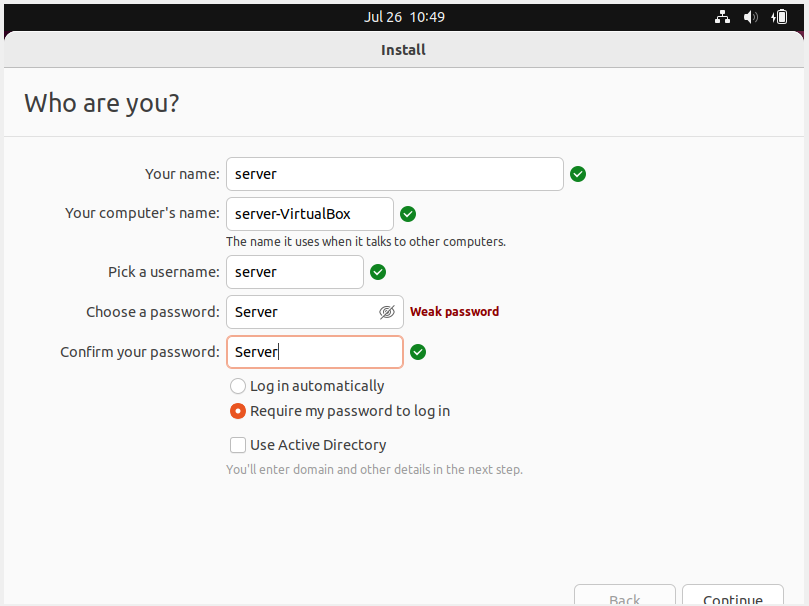
\includegraphics[width=.8\linewidth]{./Images/login_page.png}
    \caption{Filled-in login page}
    \label{fig:LoginPage}
\end{figure}


%_____________________________________________________________%

\subsection{Provide secure remote access to the VMs}
\label{sec:org1e09e96}

In the terminal of each VM, install \texttt{openssh-server} by executing the following command:
\begin{minted}[]{sh}
    sudo apt-get install openssh-server
\end{minted}

Then, go to:
\begin{minted}[]{sh}
    cd /etc/ssh
    sudo chmod 777 sshd_config
    nano sshd_config
\end{minted}

In \texttt{sshd\_config}, unmask the line: 
\begin{minted}[]{sh}
    #PasswordAuthentication yes
\end{minted}
by changing it to:
\begin{minted}[]{sh}
    PasswordAuthentication yes
\end{minted}
Type C-o to save, then C-x to leave. \newline


In the home directory of your host (your computer), generate a public key:
\begin{minted}[]{sh}
    ssh-keygen -t rsa -b 4096
\end{minted}

And send it to the VMs:
\begin{minted}[]{sh}
    ssh-copy-id -p 3333 server@localhost
    ssh-copy-id -p 2222 middlebox@localhost
    ssh-copy-id -p 1111 client@localhost
\end{minted}

In the terminal of each VM, disable the password:
\begin{minted}[]{sh}
    sudo passwd -d <username>
\end{minted}

%_____________________________________________________________%

\subsection{Allow shared folders}
\label{sec:org49c0a3b}

On the VMs, run:
\begin{minted}[]{sh}
    sudo apt-get install virtualbox-guest-x11
    sudo usermod -aG vboxsf <username>
\end{minted}

%_____________________________________________________________%

\subsection{Enhance graphical performance and integration of the VMs}
\label{sec:org22a38f4}



For each VM:
\begin{itemize}
    \item In Users, enable automatic login (Figure \ref{fig:settings}).
    \item Adjust the screen size according to your display, particularly for the client VM. (Figure \ref{fig:resolution}).
\end{itemize}

\begin{figure}[H]
    \centering
    
    \begin{subfigure}{.4\textwidth}
        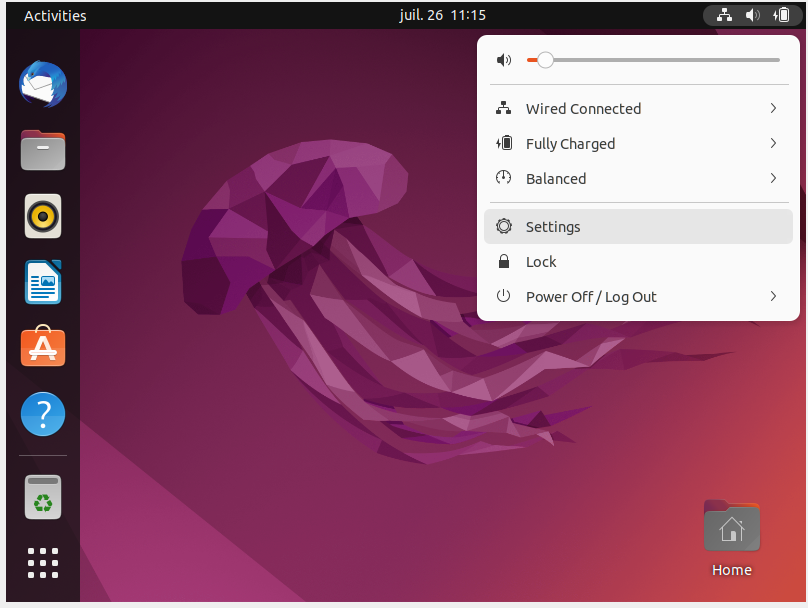
\includegraphics[width=\linewidth]{./Images/settings.png}
        \caption{Settings tab}
    \end{subfigure}
    \hfill
    \begin{subfigure}{.4\textwidth}
        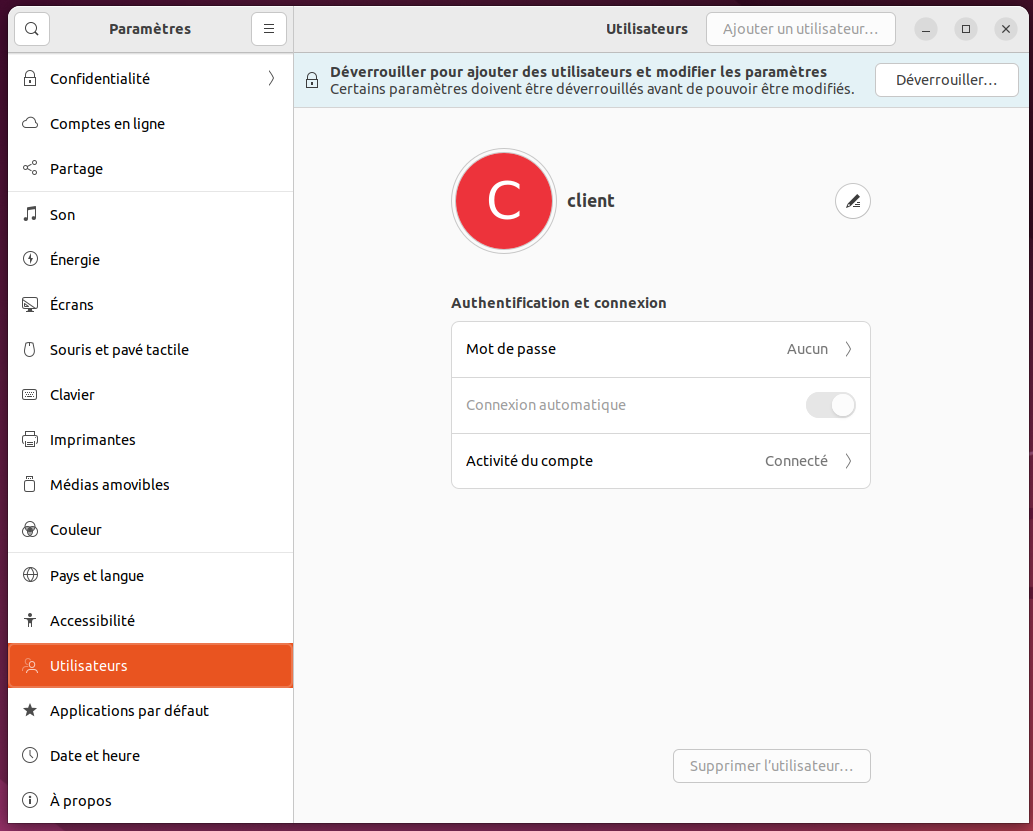
\includegraphics[width=\linewidth]{./Images/users.png}
        \caption{Users tab}
    \end{subfigure}
    \caption{Enabling automatic login}
    \label{fig:settings}
\end{figure}


\begin{figure}[H]
    \centering
    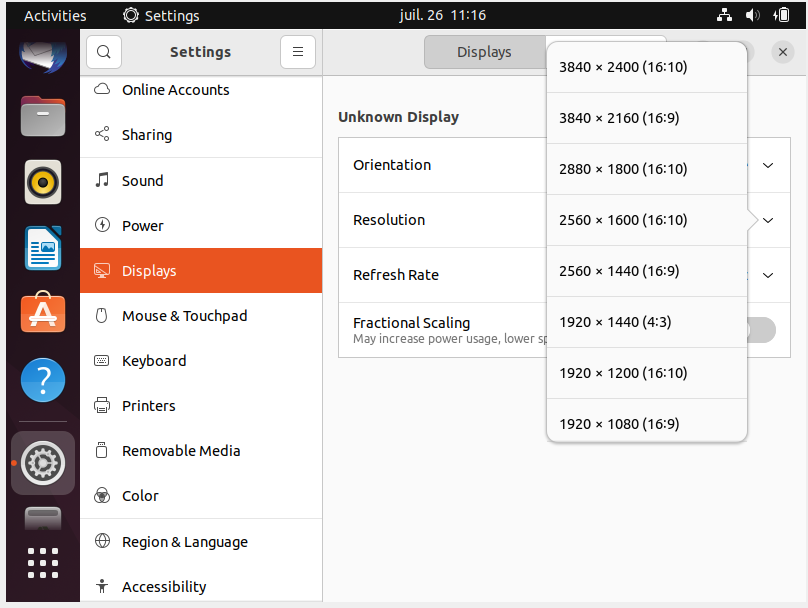
\includegraphics[width=.8\linewidth]{./Images/resolution.png}
    \caption{Resolution tab}
    \label{fig:resolution}
\end{figure}

%_____________________________________________________________%

\subsection{Upload the video files in the server VM}
\label{sec:org9db713d}

On the host, in the working directory of your wehe package, run:

\begin{minted}[]{sh}
    scp -P 3333 -r dash server@localhost:~
\end{minted}

On the server VM, move the file to the location \texttt{/var/www}:
\begin{minted}[]{sh}
    cd /home/server
    sudo mkdir /var/www
    mv dash /var/www
\end{minted}

%_____________________________________________________________%

\subsection{Finish the installation}
\label{sec:orge04b516}

On the host, run:
\begin{minted}[]{sh}
    sh wehe_demonstrator/script/manual_install2.sh
\end{minted}

On each VM, run:
\begin{minted}[]{sh}
    cd /home/<username>
    sh manual_install_<username>.sh
\end{minted}

Say yes to all and allow wireshark for non superusers. If for the server VM, you are asked to fill DNs, fill with blank values.

\clearpage
%_____________________________________________________________%
%_____________________________________________________________%

\section{Use}
\label{sec:org12ef94c}

%_____________________________________________________________%

\subsection{Launch the demonstrator}
\label{sec:orge2c8ddf}

On host, run:
\begin{minted}[]{sh}
    python3 wehe_demonstrator/src/hmi.py
\end{minted}

It takes approximately 2 minutes to start.

%_____________________________________________________________%

\subsection{Standard use}
\label{sec:org4e04f3b}

\begin{figure}[H]
    \centering
    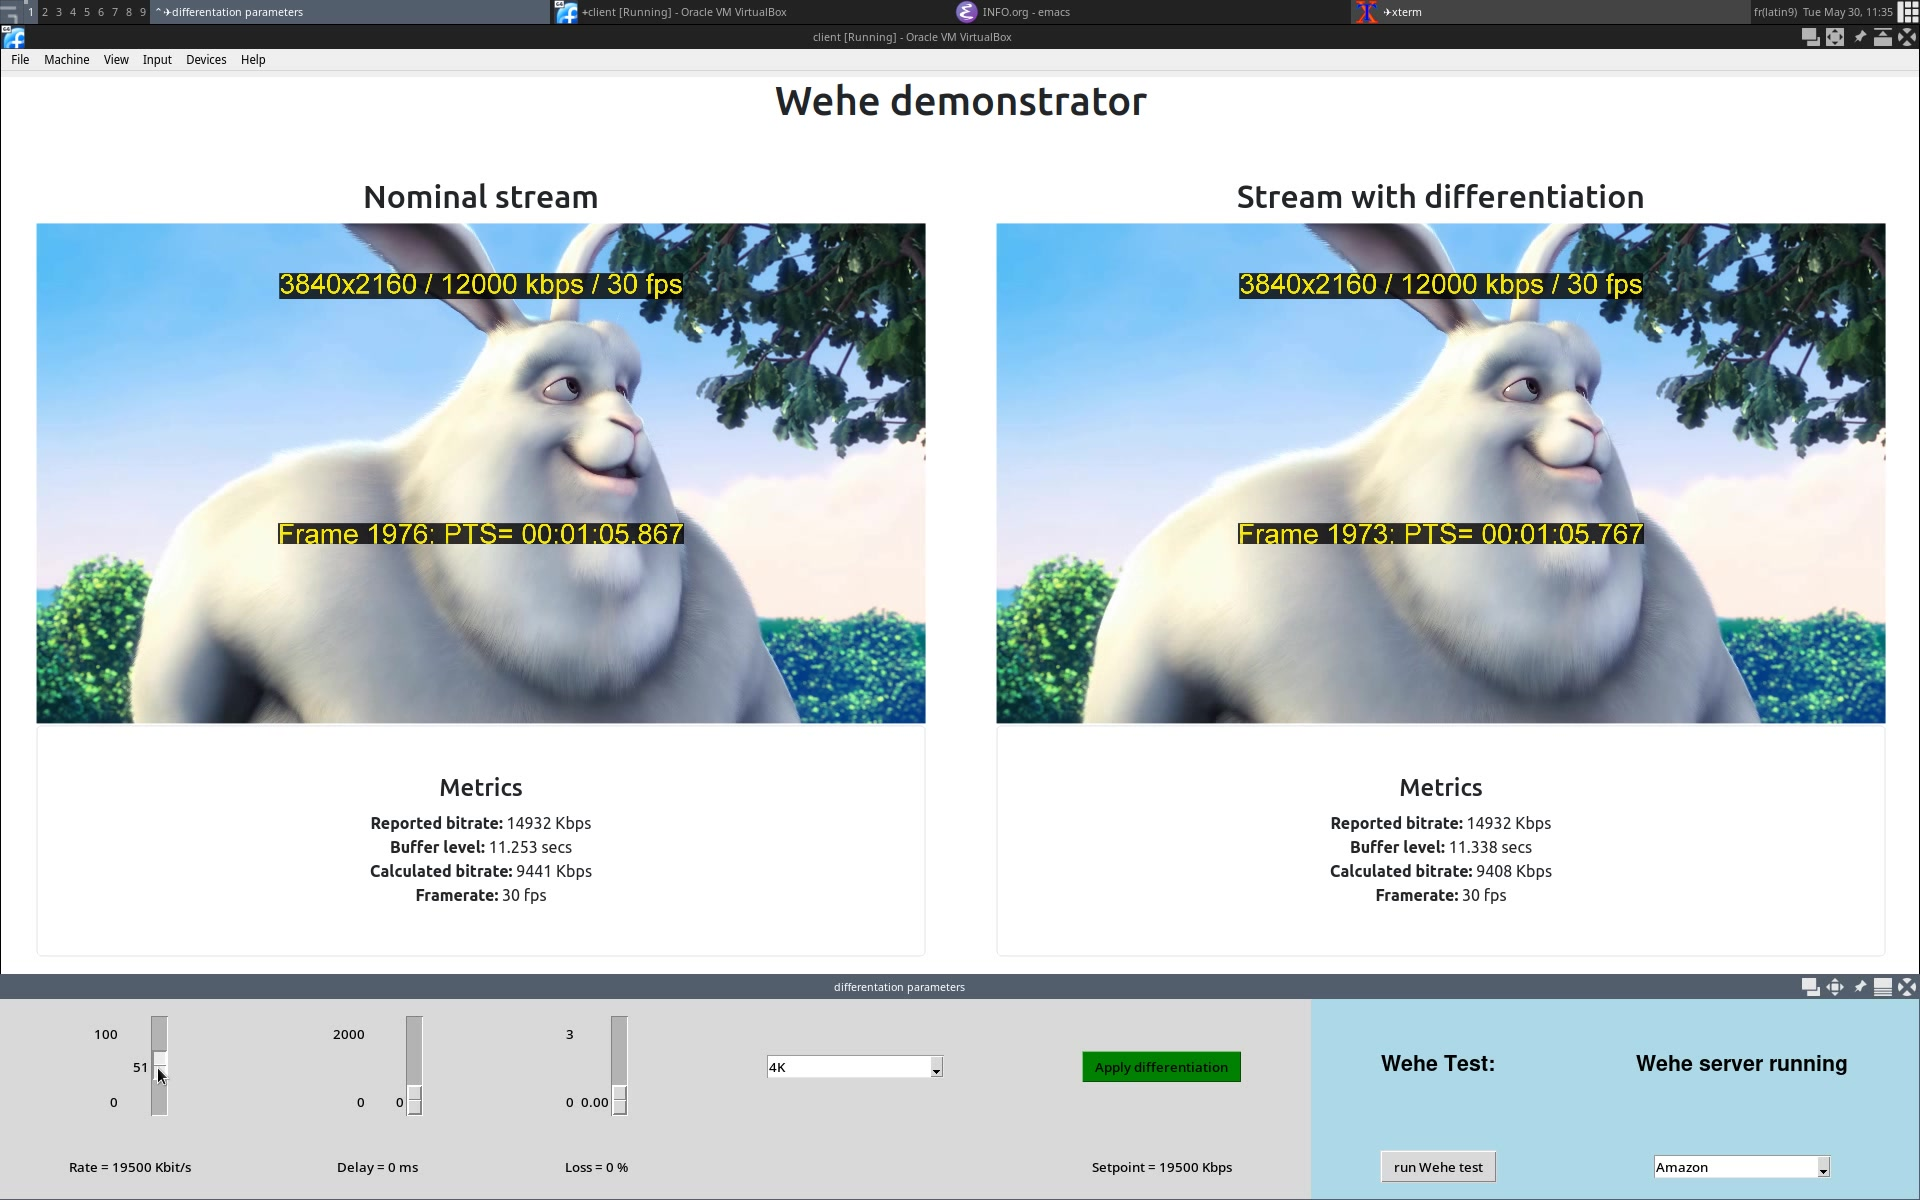
\includegraphics[width=.9\linewidth]{./Images/frame1.jpg}
    \caption{Screenshot of the application}
    \label{fig:application}
\end{figure}

In the central combobox (Figure \ref{fig:application}):
\begin{itemize}
    \item Select the nominal resolution.
    \item Select the desired differentiation with the scales for \texttt{Rate}, \texttt{Delay} and \texttt{Loss}.
    \item Click on the \texttt{Apply differentiation} button.
    \item Click on the  \texttt{run Wehe test} button.
\end{itemize}

\clearpage

%_____________________________________________________________%
%_____________________________________________________________%


\section{Check the maximum bandwidth between the server and the client}
\label{sec:org13bbf7b}

%_____________________________________________________________%

\subsection{Server side}
\label{sec:orge4451a3}

Set up a listener: 
\begin{minted}[]{sh}
    nc -l -p <port> < /dev/zero
\end{minted}

Run an IP traffic monitor:
\begin{minted}[]{sh}
    sudo apt-get install iptraf
    sudo iptraf
\end{minted}



%_____________________________________________________________%

\subsection{Client side}
\label{sec:org2dd475e}

Communicate with the server:
\begin{minted}[]{sh}
    telnet <server ip_adress> <port>
\end{minted}

\end{document}

